\chapter{Documento de Requisitos}\label{cap:06requisitos}

\section{Introducción}




%R.I%%%%%%%%%%%%%%%%%%%%%%%%%%%%%%%%%%%%%%%%%%%%%%%%%%%%%%%%%%%%%%%%%%%%%
%\section{Requisitos de Información}


%R.F%%%%%%%%%%%%%%%%%%%%%%%%%%%%%%%%%%%%%%%%%%%%%%%%%%%%%%%%%%%%%%%%%%%%%
\section{Requisitos funcionales}

\subsection{Diagrama de casos de uso}

\begin{figure}[H]
    \centering
    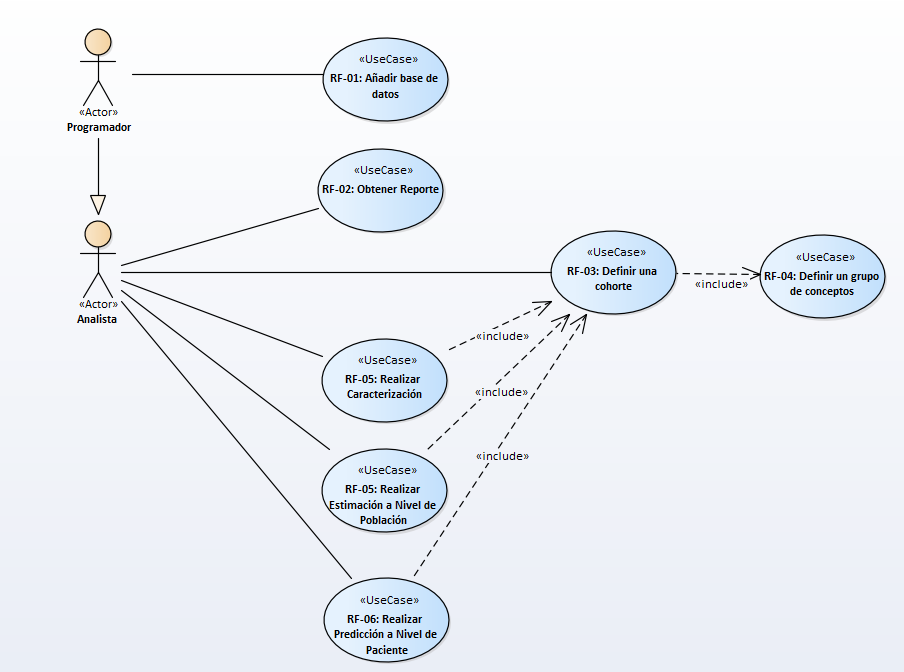
\includegraphics[width=0.90\textwidth]{figures/draftDiagramaCasosUso.png}
    \caption{Boceto de diagramas de casos de uso}
    \label{fig:draftDiagramaCasosUso}
\end{figure}

\subsection{Casos de uso}

- RF01: Cargar datasets

- RF02: Obtener un reporte del data set (Data source)

- RF03 : Definir conjuntos de conceptos del Vocabulario (Concept set)

- RF04: Configurar la muestra de trabajo (cohort definition)

- RF05: Caracterizar el cohort (characterization - primer gran bloque de metodología de OHDSI)

- RF06: Definir una etsimacion a nivel de poblacion (estimation - segundo gran bloque de metodologia de OHDSI)

- RF07: Hacer una prediccion a nivel de paciente (prediction - tercer gran bloque de metodologia de OHDSI)



%Más cosas que se pueden hacer y no definimos la otra vez:

%- Obtener un reporte de la ruta del cohorte (cohort pathway)

%- Analizar los ratios de incidencia de un outcome (INcidence rate)

%- Obteenr un reporte de los datos para un paciente concreto (profile)





%\subsection{Diagramas de casos de uso}
%\subsection{¿¿¿¿¿Descripción del requisito funcional????}


%\section{Modelo conceptual}%%%%%%%%%%%%%%%%%%%%%%%%%%%%%%%%%%%%%%%%%%%%%%

%\section{Mockups}%%%%%%%%%%%%%%%%%%%%%%%%%%%%%%%%%%%%%%%%%%%%%%%%%%%%%%%%

%R.N.F%%%%%%%%%%%%%%%%%%%%%%%%%%%%%%%%%%%%%%%%%%%%%%%%%%%%%%%%%%%%%%%%%%%%

\section{Requisitos no funcionales}


\section{Conclusiones}

En este capítulo concluimos que...
